\documentclass[11pt,letterpaper]{article}
\usepackage[margin=1in]{geometry}
\usepackage{amsmath,amssymb,booktabs,graphicx,xcolor}
\usepackage[colorlinks=true,linkcolor=blue!50!black,citecolor=blue!50!black,urlcolor=blue!50!black]{hyperref}

\newcommand{\TrainSteps}{4{,}000}
\newcommand{\PrimaryDelta}{+0.144}
\newcommand{\MeanControl}{2.548}
\newcommand{\MeanExpanded}{2.404}
\newcommand{\DeleteLow}{+0.004}
\newcommand{\DeleteHigh}{+0.271}
\newcommand{\MeanWidthGain}{+0.526}
\newcommand{\WidthEntropySlope}{+0.109}
\newcommand{\WidthLow}{+3.220}
\newcommand{\WidthHigh}{-1.715}
\newcommand{\EntropyRankLow}{0.52}
\newcommand{\EntropyRankHigh}{0.72}
\newcommand{\DiceNarrowLow}{54.82}
\newcommand{\DiceNarrowHigh}{89.14}
\newcommand{\SourceNarrowLow}{20.63}
\newcommand{\SourceNarrowHigh}{51.72}
\newcommand{\DiceWideLow}{58.04}
\newcommand{\DiceWideHigh}{87.42}
\newcommand{\SourceWideLow}{20.90}
\newcommand{\SourceWideHigh}{49.68}
\newcommand{\DiceNearestLow}{52.79}
\newcommand{\DiceNearestHigh}{54.64}
\newcommand{\SourceNearestLow}{10.95}
\newcommand{\SourceNearestHigh}{14.80}
\newcommand{\DiceLabelLow}{47.62}
\newcommand{\DiceLabelHigh}{47.62}
\newcommand{\SourceLabelLow}{0.00}
\newcommand{\SourceLabelHigh}{0.00}

\newcommand{\PrimaryRows}{%
ZCOOL KuaiLe & 16 & 1.699 & 1.522 & +0.177 \\
Long Cang & 16 & 3.270 & 2.976 & +0.293 \\
ZCOOL KuaiLe & 32 & 1.896 & 1.855 & +0.041 \\
Long Cang & 32 & 3.329 & 3.265 & +0.065 \\
}


\title{\vspace{-1em}\textbf{Generating Chinese Characters from Gaussian Noise}\\[.55em]
\large What model width changes when a glyph is hard to recover}
\author{Rain Piao\\[-2pt]\small Zisheng \enspace\textbar\enspace UCLA STATS 100A Honors}
\date{November 19, 2026}

\begin{document}
\maketitle

When I select \emph{hua}, the character for flower, the demo opens on a square of Gaussian noise. The label tells the model which character to draw. Over 1,000 steps, it looks at the current image, estimates the noise in it, and uses that estimate to take another step toward a clean image. By step 750, the lower strokes are visible in the noise. In the final frame of Figure~\ref{fig:hua}, the short marks at the top are clear as well.

\begin{figure}[ht]
\centering
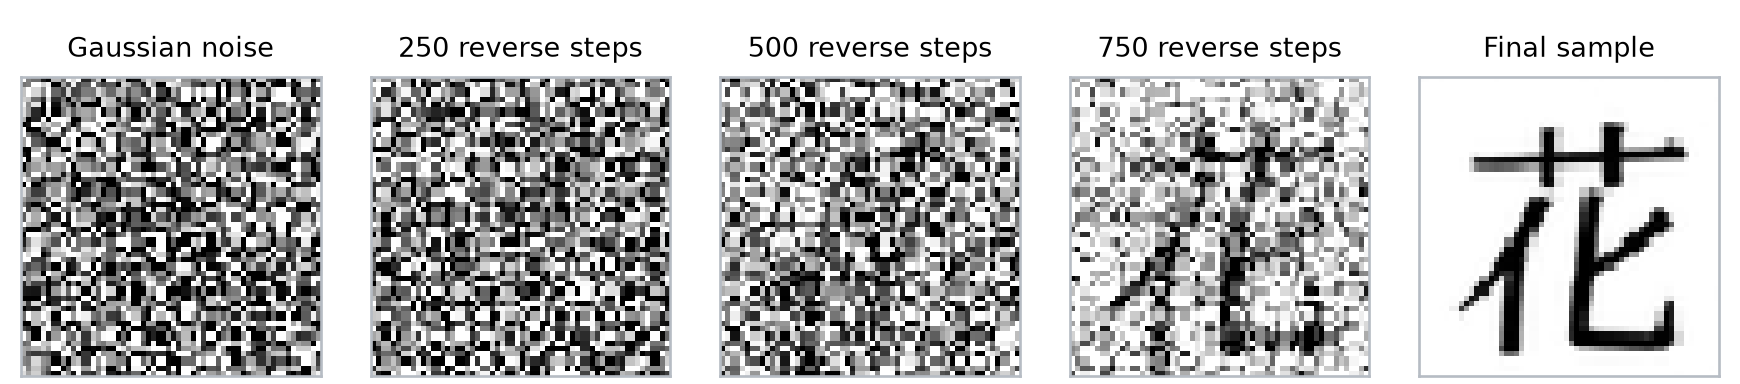
\includegraphics[width=\linewidth]{generated/pilot-hua.png}
\caption{Five saved states of one generated \emph{hua} from the original 12-character demo, sample 1 at seed 43. Each frame comes from the same reverse chain.}
\label{fig:hua}
\end{figure}

The model is a denoising diffusion probabilistic model (DDPM). To train it, I start with clean character images and add Gaussian noise at different strengths. The network sees the resulting image, the noise level, and the character label. I already know the noise I added, so I can grade its estimate and update its weights. The demo reuses that skill in reverse, starting with a fresh random draw and gradually forming a character.

What interests me is the last bit of detail. At \(48\times48\) pixels, a small gap can separate two strokes. If the gap fills in or a short mark fades, I may still read the intended character even though its shape has changed. A wider network has more channels in which to represent edges, corners, and the arrangement of strokes. I wanted to know when those extra channels actually help. The original demo gives me an example at one width. To compare two widths, I need a clean image I can use to check each answer.

\clearpage
\section*{A test with a known original}

I start with a clean drawing of a character in a particular font, save that original for scoring, and add noise to a copy. Both models get exactly the same noisy copy and character label. Figure~\ref{fig:width-example} shows two renderings of \emph{xiao}, the character for \emph{laugh}. In the stronger noise condition the short marks at the top of the glyph blur together. Under less noise the estimates preserve more of those marks and the shape of the lower strokes.

\begin{figure}[ht]
\centering
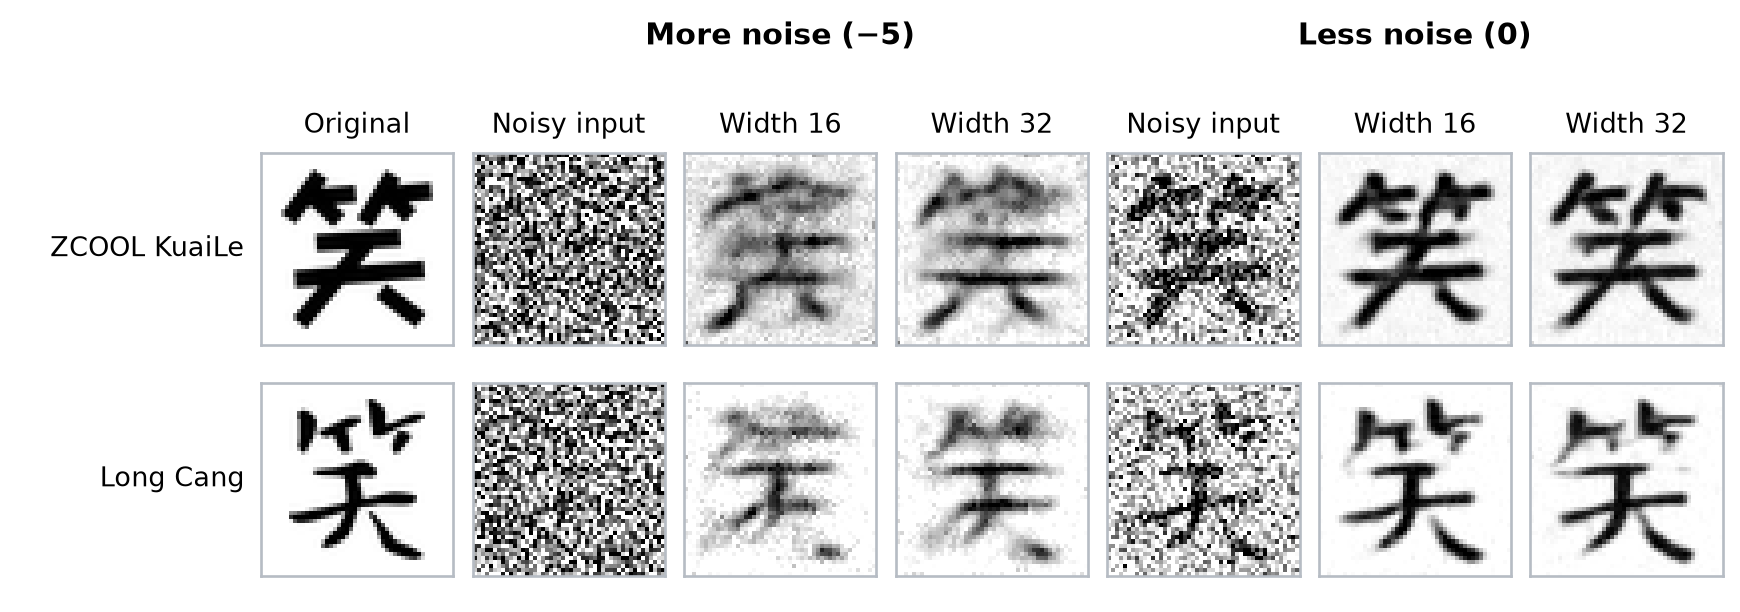
\includegraphics[width=\linewidth]{generated/width-example.png}
\caption{One scored \emph{xiao} example in each test font. Within each noise group, widths 16 and 32 use the same input. The illustration uses training seed 101 and noise draw 0. The results aggregate all 24 characters.}
\label{fig:width-example}
\end{figure}

Width is the number of feature channels in the first layer of the U-Net, the network that predicts noise. I compare 16 channels (240,993 parameters) and 32 channels (881,153 parameters). Both widths see the same training examples and use the same number of updates. The 24 character labels appear in training, and the two fonts in Figure~\ref{fig:width-example} are reserved for testing. \emph{Hua} is from the earlier demo. The two-width experiment uses the balanced 24-character set that includes \emph{xiao}.

Each model makes a single estimate of the original from a noisy input. That gives me a direct comparison with the saved original. I score the ink pixels with foreground Dice, an overlap measure from 0 to 1. If the original and prediction each have 10 ink pixels and share 8 of them, Dice is \(0.8\). The six noise levels are specified by the base-two log of the signal-to-noise ratio (SNR). At \(-5\), the signal weight squared is about \(1/32\) of the noise weight squared. At \(0\) the two weights squared are about equal.

\clearpage
\section*{When the wider model helped}

At the strongest noise level, the wider model scored \(3.22\) Dice points higher. At the mildest, it scored \(1.71\) points lower. One point equals \(0.01\) on the Dice scale. The average over all six levels was \(+0.53\) points. The left panel of Figure~\ref{fig:curves} shows why the average is hard to use on its own. A larger model was more helpful when most of the shape was buried in noise. With more of the original visible, the smaller model did a little better on this comparison.

\begin{figure}[ht]
\centering
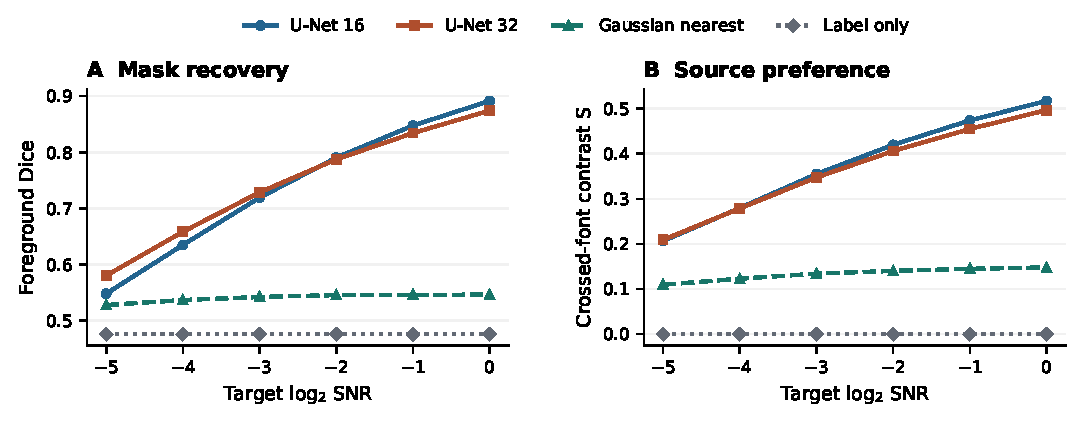
\includegraphics[width=.97\linewidth]{generated/curves.pdf}
\caption{Moving right means less noise. The left panel shows ink overlap. The right shows the advantage of matching an estimate to its own original over another rendering of the same character. The model lines average over two training seeds.}
\label{fig:curves}
\end{figure}

The distinction between overlap and source detail matters for interpreting those scores. A fixed template made from the training fonts earned \(\DiceLabelLow\) Dice points by getting the shared shape right. Its preference for the actual source was zero because it outputs the same image for either input. The denoisers' predictions did favor their own inputs. At width 32 the source advantage rose from about \(0.209\) to \(0.497\) as noise decreased.

Two characters with the same stroke count can arrange their ink very differently. I added the variety of small edge patterns to a prediction that already used stroke count, ink fraction, and perimeter complexity. The error fell from \(\MeanControl\) to \(\MeanExpanded\) Dice points. I also checked whether edge entropy predicted where extra width would help. In that fit, one standard deviation more entropy was associated with about \(0.11\) Dice points of gain from the wider model, after accounting for the other shape measures. To estimate how much capacity a more complex glyph needs, I would need a fixed recovery target and several more widths and glyphs.

\clearpage
\section*{How the comparison was scored}

The data contain six characters in each of four stroke groups (4, 6, 8, and 10). Three font families supply training images, one supplies validation images, and two supply test images. I compare both widths at two paired seeds, using \(\TrainSteps\) updates of 24 images per run and 16 test noise draws per character and font, shared across widths, seeds, and noise levels. Given clean image \(x_0\), noise \(\epsilon\sim\mathcal N(0,I)\), and a schedule weight \(a_t=\prod_{s=1}^t(1-\beta_s)\), I form \(x_t=\sqrt{a_t}x_0+\sqrt{1-a_t}\epsilon\). A trained DDPM supplies \(\widehat\epsilon\) \cite{ho2020ddpm}. The scored estimate is \(\widehat x_0=(x_t-\sqrt{1-a_t}\widehat\epsilon)/\sqrt{a_t}\).

Let \(A\) and \(B\) be the clean ink masks in the two test fonts, and \(P_A,P_B\) their predictions after thresholding. I compare each prediction with both originals using Dice \(D\). The source advantage is
\[
S=\tfrac12\bigl[D(P_A,A)-D(P_A,B)+D(P_B,B)-D(P_B,A)\bigr].
\]
The label-only template returns the same image for both inputs, so the terms cancel. The other template baseline, Gaussian nearest, chooses a training glyph \(T\) for which \(\sqrt{a_t}T\) is closest to the noisy input in squared pixel distance.

For local edge entropy, I slide a \(2\times2\) window across the ink mask, retain the 14 patterns containing both ink and background, and compute \(H=-\sum_i p_i\log_2p_i\), where \(p_i\) is pattern \(i\)'s share of the retained windows \cite{shannon1948}. Prior work has used stroke groups to compare Chinese font generation and local entropy to select reference glyphs \cite{yang2024fontdiffuser,matsuo2026active}. I take medians across training fonts for \(H\), ink fraction, and perimeter complexity. Within each test font and width I hold out one character at a time. I fit ridge regressions on the other 23 using stroke-group intercepts and standardized shape features, first without and then with \(H\).

\begin{table}[ht]
\centering
\small
\begin{tabular}{lrrrr}
\toprule
Test font & Width & MAE without \(H\) & MAE with \(H\) & Drop in MAE \\
\midrule
\PrimaryRows
\bottomrule
\end{tabular}
\caption{Mean absolute prediction error (MAE), in Dice points. The drop ranged from \(\DeleteLow\) to \(\DeleteHigh\) after removing one character and refitting.}
\end{table}

The \href{https://github.com/Rainnnee/zisheng/tree/codex/glyph-entropy-study/report/glyph-entropy}{project folder} links to the companion learning notes, trained weights, frozen protocol, and independent audit.

{\small
\bibliographystyle{unsrt}
\bibliography{references}
}

\end{document}
